También en este problema, un buen punto de partida para resolver el problema es rootear el árbol arbitrariamente:
\begin{figure}[h!]
	\centering
	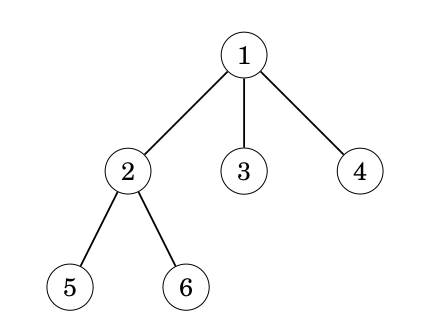
\includegraphics[width=0.4\linewidth]{img/all_longest_paths_2}
	
	\label{fig:alllongestpaths2}
\end{figure}
La primera parte del problema es calcular para cada nodo $x$ la longitud máxima de una ruta que pasa por un hijo de $x$. Por ejemplo, la ruta más larga del nodo $1$ pasa por su hijo $2$:

\begin{figure}[h!]
	\centering
	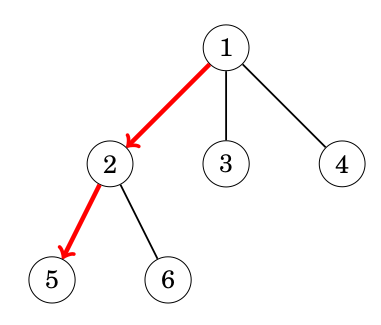
\includegraphics[width=0.4\linewidth]{img/all_longest_paths_3}
	
	\label{fig:alllongestpaths3}
\end{figure}

Esta parte es fácil de resolver en el tiempo O($N$), porque podemos usar la programación dinámica.

Luego, la segunda parte del problema es calcular para cada nodo $x$ la longitud máxima de una ruta a través de su padre $p$. Por ejemplo, la ruta más larga del nodo $3$ pasa por su padre $1$:

\begin{figure}[h!]
	\centering
	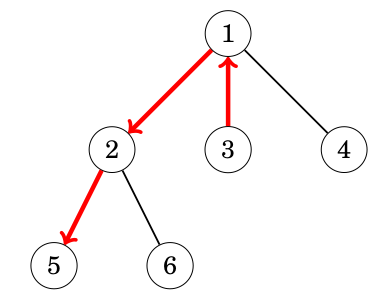
\includegraphics[width=0.4\linewidth]{img/all_longest_paths_4}
	
	\label{fig:alllongestpaths4}
\end{figure}

A primera vista, parece que debemos elegir el camino más largo desde $p$. Sin embargo, esto no siempre funciona, porque el camino más largo de $p$ puede pasar por $x$. Aquí hay un ejemplo de esta situación:

\begin{figure}[h!]
	\centering
	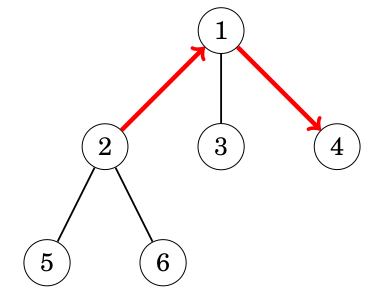
\includegraphics[width=0.4\linewidth]{img/all_longest_paths_5}
	
	\label{fig:alllongestpaths5}
\end{figure}

Aún así, podemos resolver la segunda parte en el tiempo O ($n$) almacenando dos longitudes máximas para cada nodo $x$:

\begin{itemize}
	\item \textbf{$maxLength_1(x)$:} La longitud máxima de una ruta desde $x$
	\item \textbf{$maxLength_2(x)$:} La longitud máxima de una ruta desde $x$ en otra dirección que la primera ruta
\end{itemize}
Por ejemplo, en el anterioranterior, $maxLength_1(1)=2$ usando la ruta $1 \rightarrow 2 \rightarrow 5$, y $maxLength_2(1)=1$ usando la ruta $1 \rightarrow 3$.

Finalmente, si la ruta que corresponde a $maxLength_1(p)$ pasa por $x$, concluimos que la longitud máxima es $maxlength_2(p)+1$, y de lo contrario la longitud máxima es la $maxLength_1(p)+1$.